%
% fig-integrand.tex
%
% (c) 2024 Prof Dr Andreas Müller
%
\begin{figure}
\centering
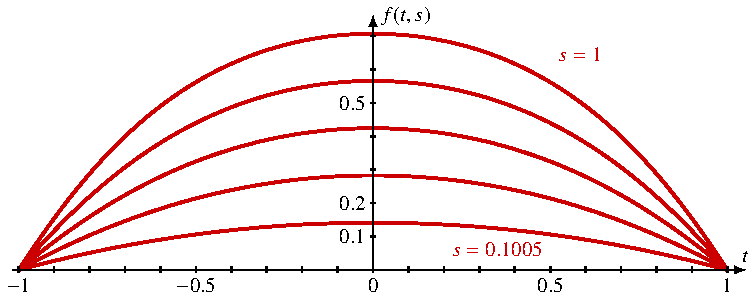
\includegraphics{chapters/030-kurvenintegral/images/integrand.pdf}
\caption{Der Integrand des Wegintegrals entlang des Weges $\gamma_s$ nimmt
das Maximum $s/\sqrt{s^2+1}$ bei $t=0$ an.
\label{buch:kurvenintegral:differential:fig:integrand}}
\end{figure}
